\chapter{Neutrinos}
%\addcontentsline{toc}{chapter}{Neutrinos}

\section{What are Neutrinos}
Neutrinos are one of the fundamental particles which make up the universe. They are also one of the least understood. Neutrinos are not affected by the electromagnetic forces because they do not have electric charge. Neutrinos are affected by a "weak" sub-atomic force of much shorter range than electromagnetism, and are therefore able to pass through great distances in matter without being affected by it. Until the late 90's, neutrinos were thought to have no mass. Due to their mass, neutrinos are also affected by gravity. Neutrinos are created by radioactive decay or nuclear reactions such as the ones that happen in the sun, in nuclear reactors or when cosmic rays hit atoms. There are three types of neutrinos, $\nu_{e}$, $\nu_{\mu}$ and $\nu_{\tau}$ which correspond to their charged lepton pairs.  

As previously stated, neutrinos are very weakly interacting; in fact, neutrinos can pass unscathed through a wall of lead several hundred light-years thick. Because neutrinos interact so rarely, studying neutrinos requires a massive detector and a powerful neutrino source. With that being said, we can only infer their existence when they interact in a detector. In a collision, distinct charged particles are produced with each type of neutrino. An electron neutrino will create an electron, a muon neutrino will create a muon, and a tau neutrino will create a tau. The track the particle leaves in the detector is how one figures out what type of neutrino interaction was “seen.” Liquid Argon Time Projection Chambers are the newest type of detectors being used to study neutrinos due to their excellent imaging and particle identification capabilities. 

\section{History of Neutrinos}
The neutrino was first postulated by Wolfgang Pauli in 1931 to explain how beta decay could resolve the conservation of energy, momentum and angular momentum problem. Pauli suggested that this missing energy might be carried off, unseen, by a neutral particle (he called neutron) which was escaping detection. James Chadwick discovered a much heavier nuclear particle in 1932 that he also named neutron, leaving two particles with the same name. Enrico Fermi was the first person to coin the term neutrino (which means little neutral one in latin) in 1933 to fix this confusion. Fermi's paper, which was published in 1934, unified Pauli's neutrino with Paul Dirac's positron and Werner Heisenberg's neutron-proton model and his theory accurately explained many experimentally observed results. Wang Ganchang first proposed the use of beta capture to experimentally detect neutrinos and in 1959 Clyde Cowan and Frederick Reines published their work stating that they had detected the neutrino. The experiment called for antineutrinos created in a nuclear reactor by beta decay that reacted with protons producing neutrons and positrons: $\nu_{e} +p^{+}\rightarrow n^{0} + e^{+}$. Once this happens, the positron finds an electron and they annihilate each other and the resulting gamma rays are detectable. The neutron is detected by neutron capture and the releasing of another gamma ray. In 1962 Leon M. Lenderman, Melvin Schwartz and Jack Steinberger were the first to detect interactions of the muon neutrino. The first detection of the tau neutrino was announced in the summer of 2000 by the DONUT collaboration at Fermilab. In the late 1960s, many experiments found that the number of electron neutrinos arriving from the sun was around $1/3$ to $1/2$ the number predicted by the Standard Solar Model. This became known as the solar neutrino problem and remained unresolved for around thirty years. This problem was resolved by the discovery of neutrino oscillation and mass.\cite{neutrino}


\section{Neutrino Oscillations}
Neutrino oscillation was first predicted by Bruno Pontecorvo. It describes the phenomenon of a neutrino created with a specific lepton flavour (electron, muon or tau) that is later measured to have a different flavour. Neutrino oscillation is important theoretically and experimentally due to the fact that this observation implies that the neutrino has a non-zero mass, which is not part of the original Standard Model of particle physics. \cite{neutrinooscillation} 

\section{Solar Oscillations and the Solar Neutrino Problem}

The solar neutrino flux derived from Bahcall's Standard Solar Model is shown in figure \ref{fig:solarmodel}. Nuclear fusion and decay processes produce an abundant amount of neutrinos. The standard solar model predicts that these reactions produce several groups of neutrinos, each with differing fluxes and energy spectra. The figure also shows the ranges of detection of existing solar neutrino experiments in different shades of blue to illustrate that they sample different portions of the solar neutrino energy spectrum. Three of these experiments, plus a new one, are discussed below.

\begin{figure}[htp]
\centering
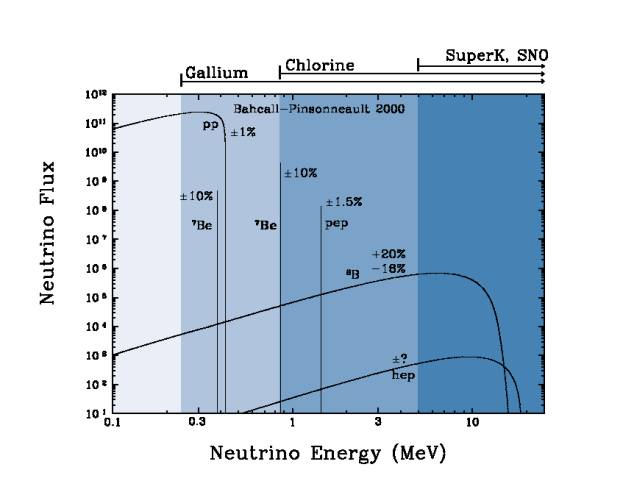
\includegraphics[scale=.55]{figs/solarmodel.jpg}
\captionof{figure}{The Standard Solar Model}
\label{fig:solarmodel}
\end{figure}

Since neutrinos rarely interact with matter, they pass through the sun and the earth undetected. About 65-billion neutrinos from the sun stream through every square centimeter on the Earth every second, yet we are oblivious to their passage in our every-day lives. \cite{bnl}

The first experiment to detect the effects of neutrino oscillation was the Ray Davis's Homestake Experiment. The detector was stationed in the Homestake Gold Mine in Lead, South Dakota. It was 1,478 meters underground and was 380 $m^{3}$. The detector was filled with perchloroethylene. Perchloroethylene was chosen because of it's high concentrations of chlorine. When an $\nu_{e}$ interaced with chlorine-37 atom, the atom would transform to argon-37 which was then extracted and counted. The neutrino capture reaction is shown in equation \ref{eq:capture}. Davis observed a deficit of about $1/3$ the flux of solar neutrinos that was predicted by Bahcall's Standard Solar Model. The unexplained difference between the measured solar neutrino flux and model predictions lead to the Solar Neutrino Problem.\cite{fnal}

\begin{equation}
\label{eq:capture}
\nu_{e} +{}^{37}Cl \rightarrow {}^{37}Ar + e^{-}
\end{equation}

While it is now known that the Homestake Experiment detected neutrinos, some physicist were weary of the results. Conclusive evidence of the Solar Neutrino Problem was provided by the Kamiokande-II experiment, a water Cherenkov detector with a low enough energy threshold to detect neutrinos through neutrino-electron elastic scattering. In the elastic scattering interaction the electrons coming out of the point of reaction strongly point in the direction that the neutrino was traveling, away from the sun. While the neutrinos observed in Kamiokande-II were clearly from the sun, there was still a discrepancy between Kamiokande-II and Homestake; The Kamiokande-II experiment measured about 1/2 the predicted flux, rather than the 1/3 that the Homestake Experiment saw.

The solution to the solar neutrino problem was finally experimentally determined by the Sudbury Neutrino Observatory(SNO). The Ray Davis's Homestake Experiment was only sensitive to electron neutrinos, and the Kamiokande-II Experiment was dominated by the electron neutrino signal. The SNO experiment had the capability to see all three neutrino flavours. Because of this, it was possible to measure the electron neutrinos and total neutrino flux. The experiment demonstrated that the deficit was due to the MSW effect,  the conversion of electron neutrinos from their pure flavour state into the second neutrino mass eigenstate as they passed through a resonance due to the changing density of the sun. The resonance is energy dependent, and is visible near 2MeV. The water cherenkov detectors only detect neutrinos above about 5MeV, while the radiochemical experiments were sensitive to lower energy (0.8MeV for chlorine, 0.2MeV for gallium), and this turned out to be the source of the difference in the observed neutrino rates at the two types of experiments. Figure \ref{fig:solarexperiments} shows Homestake, Kamiokande-II and SNO experiments. 
\begin{figure}[htp]
\centering
	\begin{subfigure}[b]{.3\textwidth}
    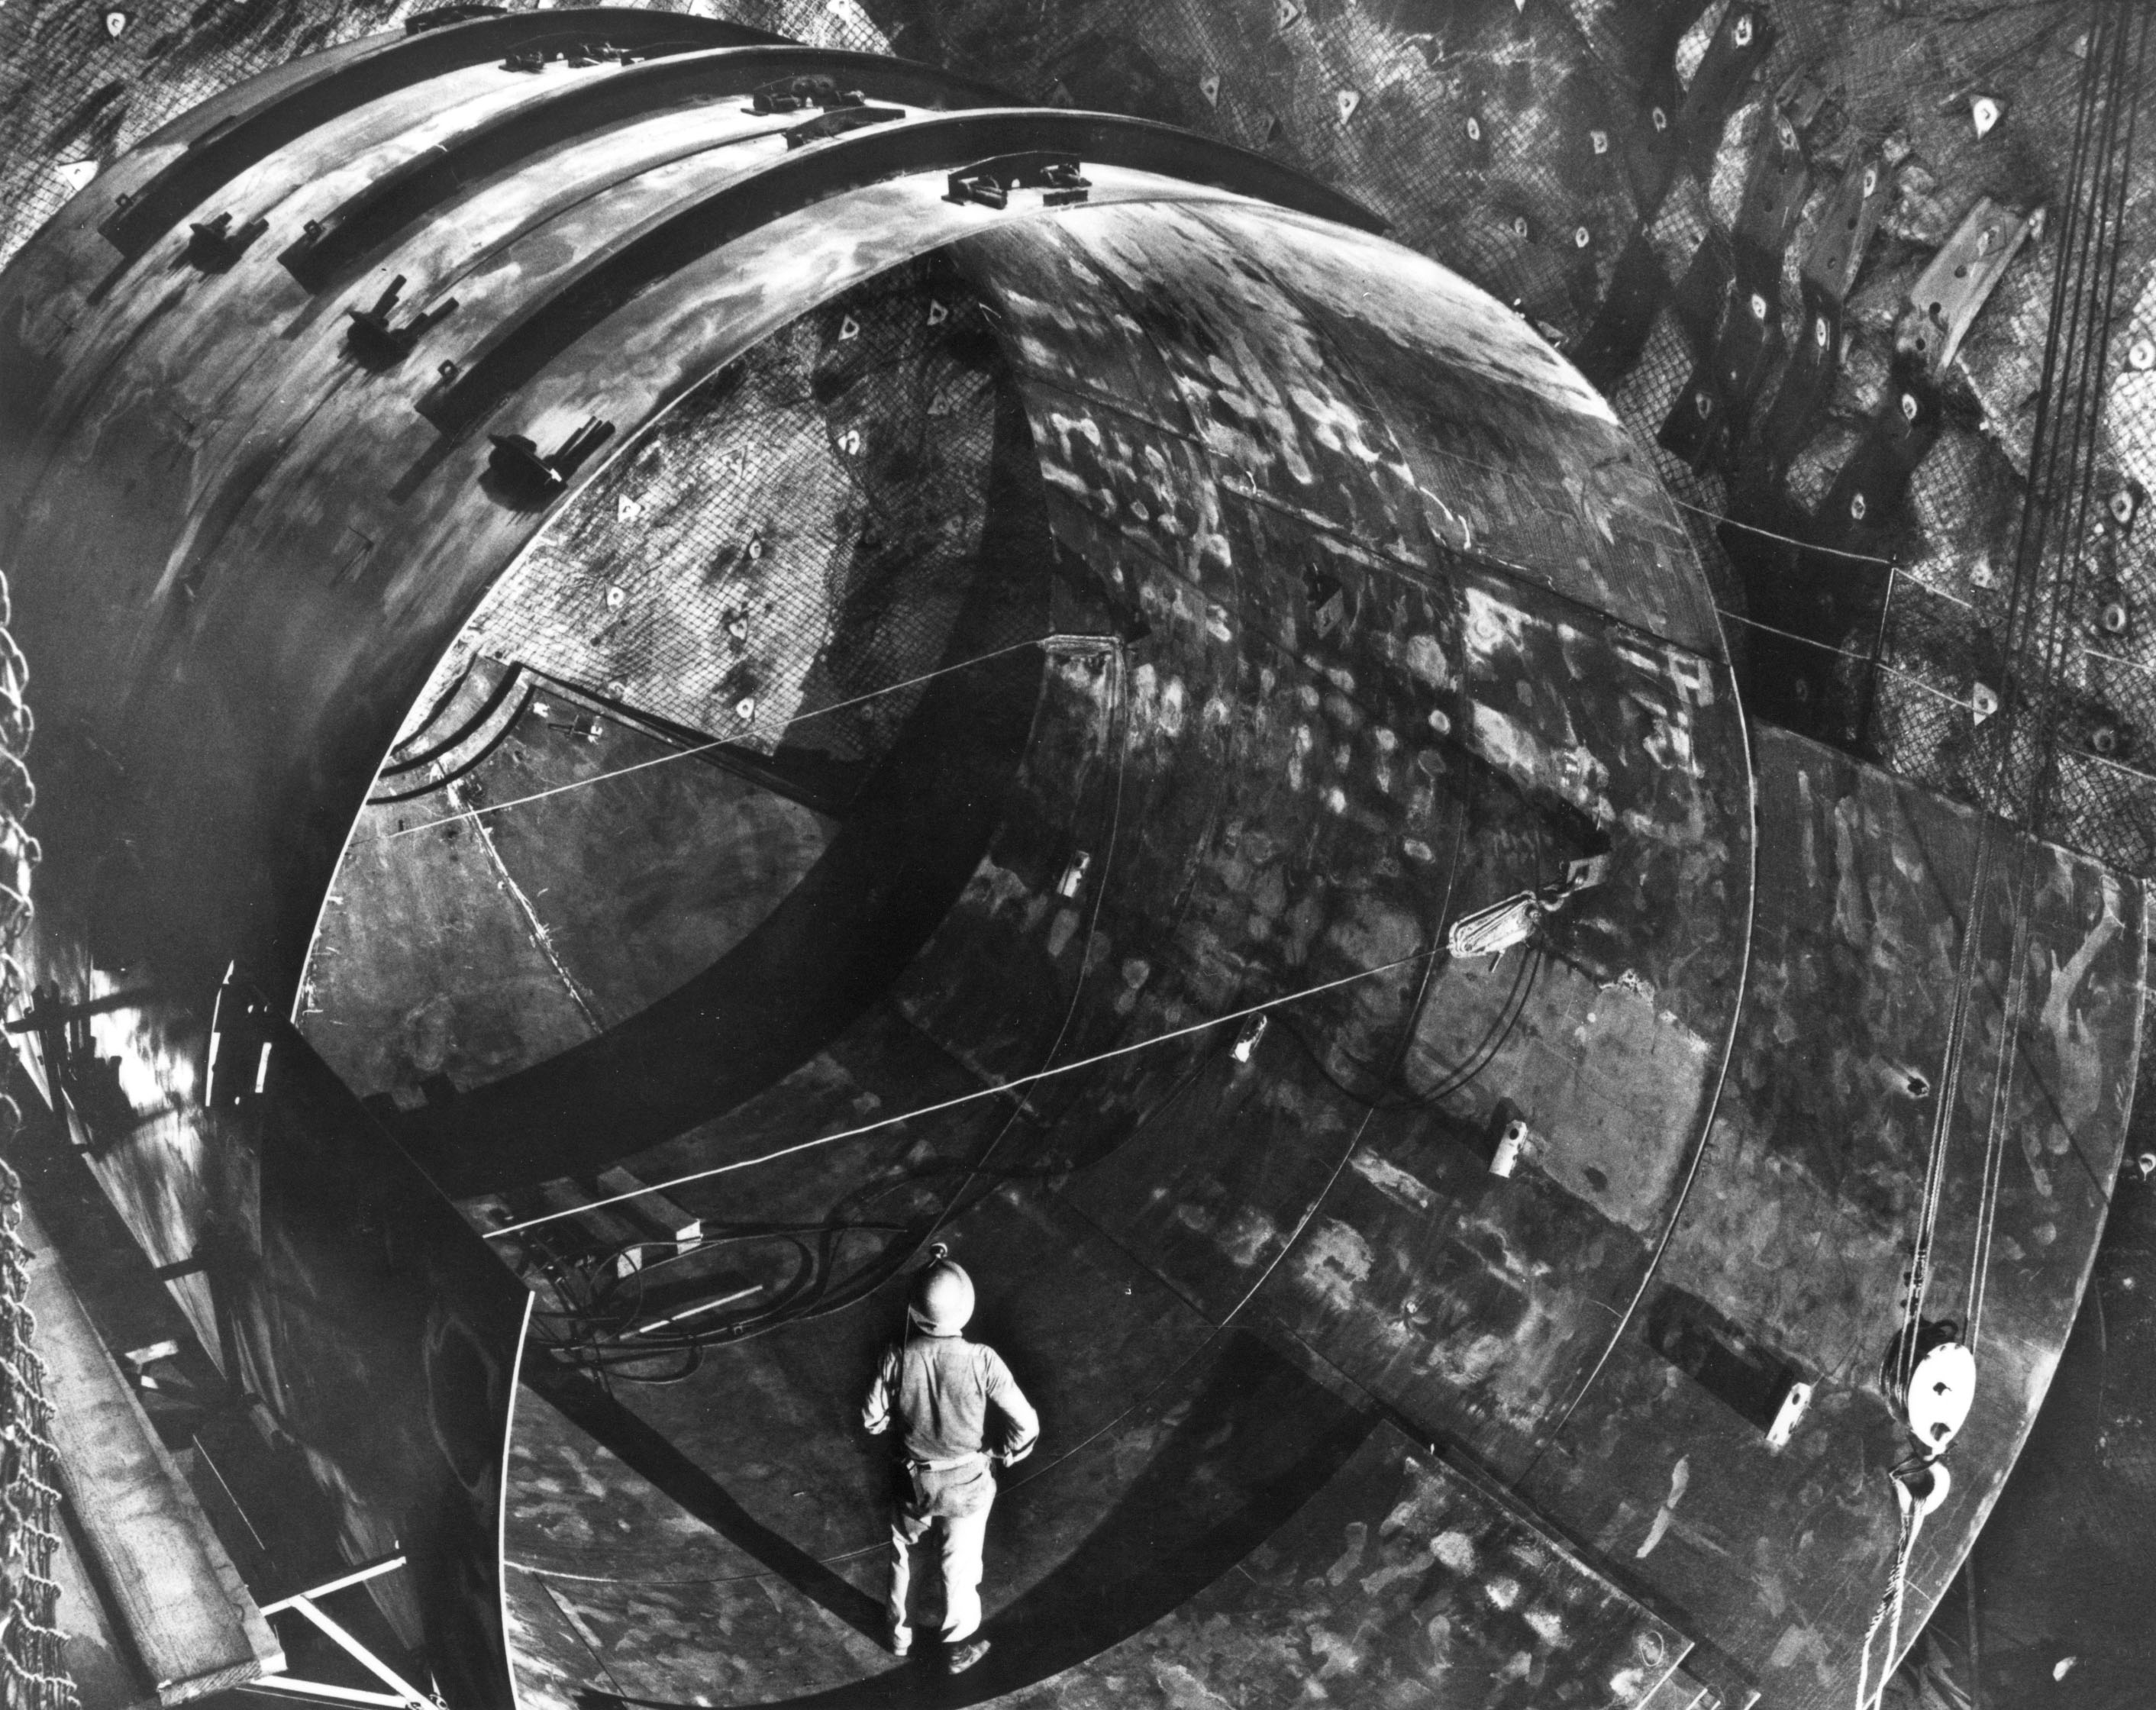
\includegraphics[width=\textwidth]{figs/homestake.jpg}
    \caption{Ray Davis's Homestake Experiment}
    \label{fig:homestake}
    \end{subfigure}
    \quad
    \begin{subfigure}[b]{.3\textwidth}
    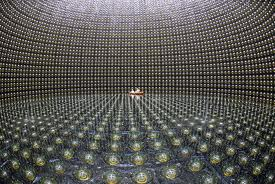
\includegraphics[width=\textwidth]{figs/kamiokande.jpg}
    \caption{Kamiokande Experiment}
    \label{fig:kamiokande}
    \end{subfigure}
    \quad
    \begin{subfigure}[b]{.3\textwidth}
    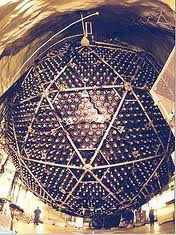
\includegraphics[width=\textwidth]{figs/sno.jpg}
    \caption{SNO Experiment}
    \label{fig:sno}
    \end{subfigure}
\caption{Solar Neutrino Experiments}
\label{fig:solarexperiments}
\end{figure}
\subsection{MSW Effect}
The Mikheyev-Smirnov-WOlfenshein effect is a process which acts to modify neutrino oscillations in matter. The presence of electrons in matter changes the energy levels of the mass eigenstates of neutrinos due to charged current coherent forward scattering of the electron neutrinos. This coherent forward scattering is similar to the electromagnetic process with respect to the refractive index of light in a medium. Because of this MSW Effect, neutrinos in vacuum have a different effective mass than neutrinos in matter and because neutrino oscillations depend on the squared mass difference of the neutrinos, the neutrino oscillations are different in matter than in vacuum. This effect is important at the sun where electron neutrinos are produced. The neutrinos of high energy leaving the sun are in a vacuum propagation eigenstate $\nu_{2}$ that has a very small overlap with the electron neutrino $\nu_{e}=\nu_{1}cos(\theta)+\nu_{2}sin(\theta)$ seen by the charged current reactions in Kamiokande-II and SNO. The discrepancy of the deficit between SNO, Kamiokande-II and Homestake is due to the energy of the solar neutrinos. The MSW effect "turns on" at about 2MeV and at lower energies, this MSW effect is negligible. \cite{Smirnov:2003da}



\section{Atmospheric Oscillations and the Atmospheric Neutrino Anomaly}
Atmospheric neutrinos are neutrinos that stem from the decay hadrons coming from primary cosmic rays. The dominant part of the decay chain is shown in equations  \ref{eq:piplus} and \ref{eq:piminus}

\begin{equation}
\label{eq:piplus}
\pi^{+} \rightarrow \mu^{+} \nu_{\mu} \mu^{+} \rightarrow e^{+} \nu_{e} \overline{\nu_{\mu}}
\end{equation}
\begin{equation}
\label{eq:piminus}
\pi^{-} \rightarrow \mu^{-} \overline{\nu_{\mu}} \mu^{-} \rightarrow e^{-} \overline{\nu_{e}} \nu_{\mu}
\end{equation}

\begin{figure}[htp]
\centering
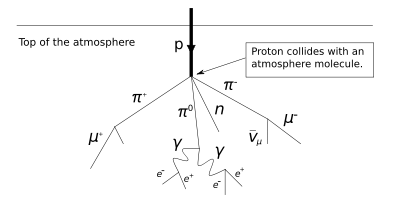
\includegraphics[scale=.5]{figs/cosmicray.jpg}
\caption{Cosmic Ray Shower}
\label{fig:cosmicray}
\end{figure}

Figure \ref{fig:cosmicray} shows the cosmic ray shower. In general, these neutrinos have energies from 1GeV to 100s of GeV and the ratio of $\nu_{\mu}$s to $\nu_{e}$s equals to 2 (see equation \ref{eq:ratio})
\begin{equation}
\label{eq:ratio}
R = \frac{(\nu_{\mu} + \overline{\nu_{\mu}})}{(\nu_{e} + \overline{\nu_{e}})}
\end{equation} 



There have been two types of detectors used to study atmospheric neutrinos: Water Cherenkov detectors and tracking calorimeters. Super-Kamiokande is the detector we will focus on. These atmospheric detector experiments measure the ratio of $\nu_{\mu}$ to $\nu_{e}$. They also measure the zenith angle distribution of the neutrinos. These experiments report a double ratio (shown in equation \ref{eq:doubleratio}). This double ratio is the ratio measured in the detector to the ratio thats expected which is 2. If the double ratio equals to 1, the data agrees with the prediction. Various measurements from multiple experiments are shown in figure \ref{fig:ratiotable}. Except for Frejus, all R measurements are less than 1. This discrepancy between the predicted R and the measured R became known as the Atmospheric Neutrino Anomaly.
\begin{equation}
\label{eq:doubleratio}
R = \frac{(N_{\mu}/N_{e})_{DATA}}{(N_{\mu}/N_{e})_{SIM}}
\end{equation}

\begin{figure}[htp]
\centering
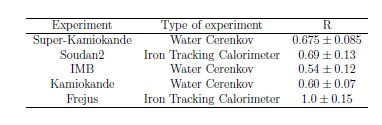
\includegraphics[scale=1]{figs/ratio.jpg}
\caption{Measurments of the double ratio for various atmospheric neutrino experiments}
\label{fig:ratiotable}
\end{figure}

Kamiokande-II has the the capability of measuring the direction of the incoming neutrinos. The expectation of atmospheric neutrino detection is that the flux be isotropic due to the fact that atmospheric neutrinos can reach the detector from all directions. Kamiokande-II noticed that muon-like data did not agree well with this expectation. At low energies approximately half of the $\nu_{\mu}$ are missing over the full range of zenith angles. At high energies the number of $\nu_{\mu}$ coming down from above the detector seems to agree with expectation, but half of the same $\nu_{\mu}$ coming up from below the detector are missing. This anomaly can be easily explained by neutrino flavour oscillations. Due to the fact that the neutrino travels less distance coming straight down into the detector (about 15km) than coming up from the bottom of the detector(13000km) changes the probability of oscillation. The probability of oscillation for the muon neutrinos coming down into the detector is roughly zero, whereas for neutrinos coming up, the oscillation probability is $sin^2(2\theta)$. Also, that fact that the electron-like events are not reduced, but the muon-like events are, suggests that the oscillation mode for atmospheric neutrinos is $\nu_{\mu} \rightarrow \nu_{\tau}$. 
Both the solar and atmospheric neutrino problems can be explained by neutrino oscillation so its fitting to derive this phenomenon mathematically. In the next two sections, two flavour and three flavour neutrino oscillation derivations will be explained. 


\section{Two Flavour Neutrino Oscillation Formulation}
The flavour eigenstates can oscillate between eachother because they are composed of an add-mixture of mass eigenstates($\nu_{1}$,$\nu_{2}$). Figure \ref{fig:mixing} shows the mass and flavour eigenstates rotated by an angle $\theta$ which is the mixing angle. 

In matrix form the wavefunctions are:

\begin{equation}
\begin{pmatrix}
\nu_{\mu} \\
\nu_{e}
\end{pmatrix} 
 = \begin{pmatrix}
cos\theta & sin\theta \\
-sin\theta & cos\theta 
\end{pmatrix}*
\begin{pmatrix}
\nu_{1} \\
\nu_{2} 
\end{pmatrix}
\end{equation}


\begin{figure}[htp]
\centering
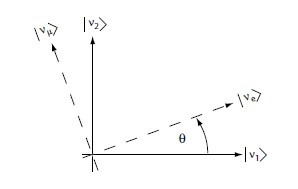
\includegraphics[scale=.8]{figs/mixingangle.jpg}
\caption{The flavour eigenstates are rotated by an angle $\theta$ with respect to the mass eigenstates}
\label{fig:mixing}
\end{figure}

Applying the time evolution operator to $\nu_{\mu}$:
\begin{equation}
\centering
\label{eq:timeevol}
|\nu_{\mu}(t)> = -sin\theta|\nu_{1}>e^{-i\frac{E_{1}t}{\hbar}} + cos\theta|\nu_{2}>e^{-i\frac{E_{2}t}{\hbar}}
\end{equation}

where $E_{1} = \sqrt{p^2 c^2 + m^2_{1} c^4}$ and $E_{2} = \sqrt{p^2 c^2 + m^2_{2} c^4}$ and $p_{1}=p_{2}$. For the time being, let us assume $\hbar=c=1$. 
With this assumption:
$E_{1}=\sqrt{p^2+m^2_{1}}$ and $E_{2} = \sqrt{p^2 + m^2_{2}}$.
The next modifications is to assume neutrinos are relativistic:
\begin{equation}
\centering
\label{eq:gamma}
\gamma = \frac{E}{m^2_{o} c^2} = \frac{\sqrt{p^2 c^2 + m^2_{o} c^4}}{m_{o} c^2} \gg 1
\end{equation}
because of this,
\begin{equation}
\centering
p \gg m_{o}
\end{equation}
\begin{equation}
\centering
E = \sqrt{p^2 + m^2_{o}}=p\sqrt{1+m^2_{o}/p^2}\simeq p + \frac{1}{2}\frac{m^2_{o}}{p}
\end{equation}

where the binomial expansion is used. Now $E_{1}$ and $E_{2}$ can be written as:
\begin{equation}
\centering
E_{1} \simeq p + \frac{1}{2}\frac{m^2_{1}}{p} \mbox{    and    }  E_{2} \simeq p + \frac{1}{2}\frac{m^2_{2}}{p}
\end{equation} 
Now applying all these assumptions back into equation \ref{eq:timeevol} gives us:
\begin{equation}
\centering
|\nu_{\mu}(t)> = -sin\theta|\nu_{1}>e^{-i\left( p+\frac{1}{2}\frac{m^2_{1}}{p}\right)t} + cos\theta|\nu_{2}>e^{-i\left(p+\frac{1}{2}\frac{m^2_{2}}{p}\right)t}
\end{equation}
\begin{equation}
\centering
|\nu_{\mu}(t)> = e^{-i \left( p+\frac{1}{2}\frac{m^2_{1}-m^2_{2}}{p} \right) t} \left( -sin\theta|\nu_{1}> + cos\theta|\nu_{2}> \right)
\end{equation}
 Substituting $\Delta m^2 = m^2_{1}-m^2{2}$ and $t = \frac{x}{c} =x$ and $e^{-iz}= e^{-i \left( p+\frac{1}{2}\frac{m^2_{1}}{p} \right) t}$ gives us:
 \begin{equation}
 \centering
 |\nu_{\mu}(t)> = e^{-iz} \left( -sin\theta|\nu_{1}> + cos\theta|\nu_{2}>e^{+ix \left(\frac{1}{2}\frac{\Delta m^2}{p}\right)}\right)
 \end{equation}

Finding the Probability for a $\nu_{\mu} \rightarrow \nu_{e}$:
\begin{equation}
\centering
P(\nu_{\mu} \rightarrow \nu_{e}) = |<\nu_{e}|\nu_{\mu}(t)>|^2
\end{equation}

Remembering that $<\nu_{i}|\nu_{j}>=\delta_{ij}$
\begin{equation}
\centering
<\nu_{e}|\nu_{\mu}(t)> = e^{-iz}\left(-sin\theta cos\theta + sin\theta cos\theta e^{\frac{i \Delta m^2 x}{p}}\right)
\end{equation}
Taking the absolute value squared gives us:
\begin{equation}
\centering
P(\nu_{\mu} \rightarrow \nu_{e}) = |<\nu_{e}|\nu_{\mu}(t)>|^2 = e^{+iz}e^{-iz}sin^{2}\theta cos^{2}\theta\left( -1 + e^{\frac{i \Delta m^2 x}{p}}\right)\left(-1 + e^{\frac{i \Delta m^2 x}{p}}\right)
\end{equation}

Since the neutrino is relativistic we can set $p= E_{\nu}$ and change $x=L$. Also recognizing the trigonometric relation $(1 - cos2\theta)/2 = sin^{2}\theta$ the above equation becomes:
\begin{equation}
\centering
P(\nu_{\mu} \rightarrow \nu_{e}) = sin^{2}2\theta sin^2\left(\frac{\Delta m^2 L}{4 E_{\nu}}\right)
\end{equation}
 
 All that's left to do now is re-introduce $\hbar$ and $c$ doing this we get:
 \begin{equation}
 \centering
 P_{\nu_{\mu} \rightarrow \nu_{e}} (L,E) = sin^{2}2\theta sin^2\left(1.27 \Delta m^2 \frac{L}{E_{\nu}}\right)
 \end{equation}
 
 This equations has three important variables. 
 \begin{itemize}
 \item The angle $\theta$: This angle, as mentioned before, is called the mixing angle. It defines the difference between the flavour and the mass eigenstates. When $\theta = 0$ the mass and flavour eigenstates are identical and now oscillations occur. 
 \item The mass squared difference, $\Delta m^2$: Again $\Delta m^2 = m^2_{1}-m^2_{2}$. The reason this is an important variable is because it implies that for neutrinos to oscillate, neutrinos must have mass. Furthermore, the mass squared difference also tells us that the neutrino mass eigenstates must be different. 
 \item L/E: This is the variable that is of most interest to experimental physicists due to the fact that it is the variable that we set. L is the distance between the source and detector and E is the energy of the neutrino. For a given $\Delta m^2$, the probability of oscillation changes with respect to L/E. 
 \end{itemize}

\section{Three Flavour Neutrino Oscillation Formulation}
Seeing the quantum mechanics involved in deriving the probability of a two flavour neutrino oscillation, it is now possible to formulate the three flavour neutrino oscillation. The three flavour neutrino oscillation formulation begins  similarly to the two flavour, but there is the Pontecorvo-Maki-Nakagawa-Sakata matrix (PMNS) instead of the 2X2 matrix in the previous section. The PMNS matrix is show below:
\begin{equation}
\centering
\begin{pmatrix}
c_{12}c_{13} & s_{12}c_{13} & s_{13}e^{-i \delta} \\
-s_{12}c_{23} - c_{12}s_{23}s_{13}e^{i \delta} & c_{12}c_{23} -s_{12}s_{23}s_{13}e^{i \delta} & s_{23}c_{13}\\
s_{12}s_{23} - c_{12}c_{23}s_{13}e^{i \delta} & -c_{12}s_{23} - s_{12}c_{23}s_{13}e^{i \delta} & c_{23}c_{13}
\end{pmatrix} *
\begin{pmatrix}
e^{i \alpha_{1}/2} & 0 & 0\\
0 & e^{i \alpha_{2}/2} & 0\\
0 & 0 &1
\end{pmatrix}
\end{equation} 
where $c_{ij}=cos\theta_{ij}$ and $s_{ij}=sin\theta_{ij}$

Following the same steps as before we get:
\begin{equation}
\centering
P_{\alpha \rightarrow \beta}= \delta_{\alpha \beta} - 4 \Sigma Re(U^{*}_{\alpha i} U_{\beta i} U{\alpha j} U^{*}_{\beta j})sin^{2}\left(\frac{\Delta m^{2}_{ij} L}{4E}\right) 2 \Sigma Im(U^{*}_{\alpha i} U_{\beta i} U{\alpha j} U^{*}_{\beta j})sin\left(\frac{\Delta m^{2}_{ij} L}{2E}\right)
\end{equation}

The main things to notice here are $\delta_{ij}$ which is the CP violating term and has not been measured yet, and $\theta_{13}$ which has just been measured. CP violation is a violation of the postulated CP-symmetry. CP-symmetry states that the laws of physics should be the same if a particle were to be exchanged with its antiparticle and then if the left hand side of a decay were switched with the right hand side. 

%\section{Reactor Oscillation}
%Many experiments have searched for oscillation of electron anti-neutrinos produced at nuclear reactors. Such oscillations give the value of the parameter θ13. The KamLAND experiment, started in 2002, has made a high precision observation of reactor neutrino oscillation. Neutrinos produced in nuclear reactors have energies similar to solar neutrinos, a few MeV. The baselines of these experiments have ranged from tens of meters to over 100 km.
%On 8 March 2012, the Daya Bay team announced a 5.2σ discovery that θ13≠0. Two other experiments are currently measuring reactor neutrino oscillation (at the same baseline of a few kilometers) and may eventually confirm the Daya Bay results: Double Chooz and RENO.


%\section{Beam Oscillation}
%Neutrino beams produced at a particle accelerator offer the greatest control over the neutrinos being studied. Many experiments have taken place which study the same neutrino oscillations which take place in atmospheric neutrino oscillation, using neutrinos with a few GeV of energy and several hundred km baselines. The MINOS experiment recently announced that it observes consistency with the results of the K2K and Super-K experiments.
%The controversial observation of beam neutrino oscillation at the LSND experiment in 2006 was tested by MiniBooNE. Results from MiniBooNE appeared in Spring 2007, and appeared to contradict the findings of the LSND experiment. Results from the HARP-CDP group also put the LSND result into doubt.
%On 31 May 2010, the INFN and CERN announced having observed a tau particle in a muon neutrino beam in the OPERA detector located at Gran Sasso, 730 km away from the neutrino source in Geneva.
%The currently-running T2K experiment uses a neutrino beam directed through 295 km of earth, and will measure the parameter θ13. The experiment uses the Super-K detector. NOνA is a similar effort. This detector will use the same beam as MINOS and will have a baseline of 810 km.


%\section{Unanswered questions about Neutrinos }
%There are many questions that haven't been answered by previous experiments. Many of them I have touched upon in previous sections, but here is a formal list of questions left unanswered. 
%\begin{itemize}
%\item What is the sign of $\Delta m^{2}_{23}$?
%\item Are there more than three active neutrinos? (LSND experiment)
%\item Are the neutrinos and antineutrinos identical?
%\item Is there a CP violating term that needs to addressed. 
%\item Will $\delta_{cp}$ explain matter-antimatter asymmetry?  
%\item Why is the PMNS matrix so different in form to the CKM matrix( quark mixing matrix)
%\end{itemize}


%\section{Final Thoughts}
%Although there is much about neutrinos that we don't know, we have made much progress in trying to understand these elusive particles. We now know that neutrinos aren't massless and because of this knowledge we now know that neutrinos oscillate between flavour and mass eigenstates. We have also just recently discovered that $\theta_{13}$ is non-zero and this knowledge will lead to experiments and data analysis to find $\delta_{cp}$.
%\clearpage

%More introduction
